\section{Self-Speculative Tool Use}
\label{sec:selfspec}

The cost model in \S\ref{sec:eq1} identifies three conditions for speculation to succeed:
high gate acceptance ($\alpha$), sufficient overlap time ($\toverlap$), and low overhead
($\Toh$).
Whether these are achievable depends on an empirical question about the model itself:

\begin{tcolorbox}[
  colback=blue!3!white,
  colframe=blue!45!black,
  boxrule=0.45pt,
  arc=1.5pt,
  left=4pt,
  right=4pt,
  top=3pt,
  bottom=3pt
]
\textbf{Research question.}
Can a running LLM predict its own next tool call \emph{accurately} enough,
\emph{early} enough, and \emph{recoverably} enough that speculative tool use
pays off?
\end{tcolorbox}

\noindent We constrain the prediction source to the running model's own
state: no auxiliary model, no historical traces.
We answer affirmatively with three empirical insights, established on
\textbf{Qwen3-32B} across five real-tool and simulated benchmarks (GAIA, HotpotQA,
tau2-bench, BrowseComp, BFCL): the model already knows its next tool call
(Insight~1, \emph{accuracy}), its own confidence signals when to commit
(Insight~2, \emph{timing}), and even rejected probes leave verified prefixes
(Insight~3, \emph{recovery}). How these properties scale to a smaller model (Qwen3-4B)
and where they break (native XML tool formats) is examined in \S\ref{sec:envelope}.

\subsection{Insight 1: Models Already Know Their Next Tool Call}
\label{sec:insight1}

A short forced-prefix probe can expose the next tool identity well before the serial tool
boundary.
We force a tool-call prefix immediately after the model's first decode token
(fork-at-start) and compare the probe's predicted tool name and arguments against the
model's unrestricted generation.

\begin{figure}[t]
  \centering
  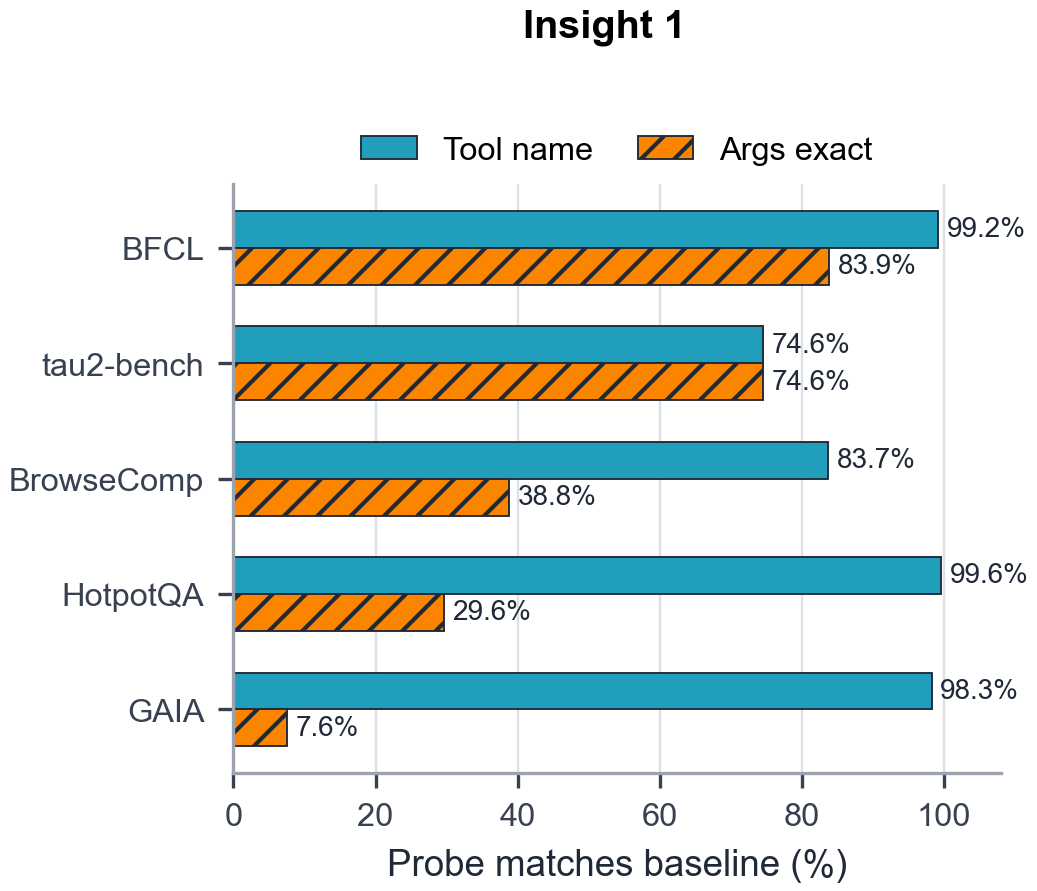
\includegraphics[width=0.95\columnwidth]{figures/fig1b_per_turn_fork_accuracy_top.png}
  \caption{\textbf{Fork-at-start probes recover the next tool name across workloads.}
  On Qwen3-32B, forced tool-call probes near decode start predict the eventual tool
  name across five benchmarks (sorted by argument exact-match; hatched bars).
  Protocols: replay pos=0 (GAIA, tau2-bench, BFCL) and online first-token
  (BrowseComp, HotpotQA).}
  \label{fig:fig1b_fork_acc}
\end{figure}

\parabf{Foresight across benchmarks.}
On Qwen3-32B, near-decode-start tool-name accuracy is consistently high across the five
benchmarks in Figure~\ref{fig:fig1b_fork_acc}: 98.3\% on GAIA, 74.6\% on tau2-bench,
83.7\% on BrowseComp, 99.6\% on HotpotQA, and 99.2\% on BFCL.
Argument-exact accuracy is lower and more variable (7.6--83.9\%), reflecting the
difficulty of predicting precise parameter values before observing the chain-of-thought.
This is the gap that Insight~2 addresses.

\parabf{No-op recovery.}
On 11 tau2-bench turns where the baseline declined to call any tool, 9/11 forced-probe
outputs were correct tool calls the model should have made; fork-prefix can act as a
cheap correction against model over-caution.

\parabf{Implication for EQ1.}
High name accuracy means $\alpha$ (gate acceptance on name match) is intrinsically high
before any confidence gating.
The remaining challenge is argument accuracy, which Insight~2 addresses.

\subsection{Insight 2: Confidence Improves with Chain-of-Thought}
\label{sec:insight2}

\begin{figure}[!t]
  \centering
  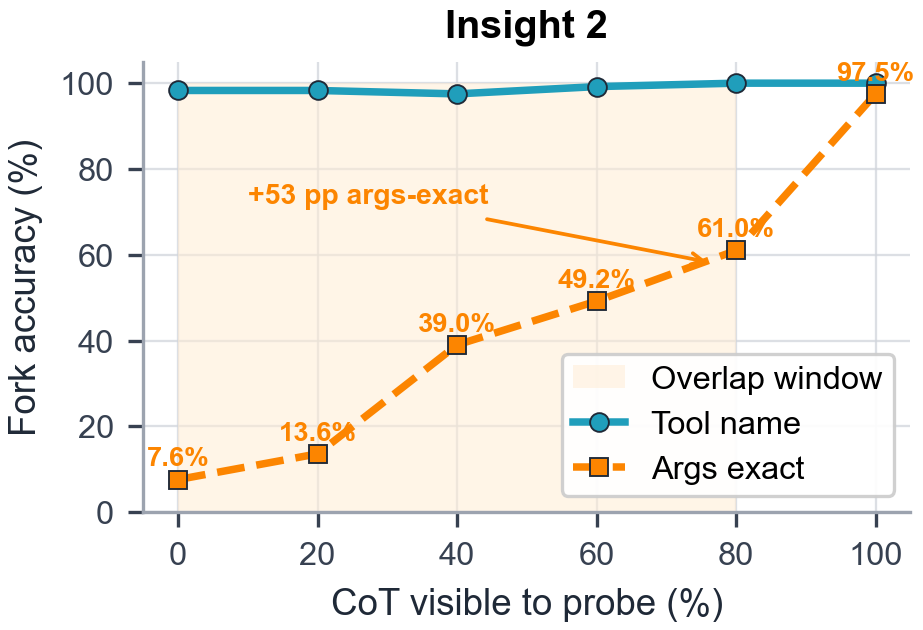
\includegraphics[width=0.93\columnwidth]{figures/fig_insight2_cot_curve_gaia.png}
  \caption{\textbf{Fork accuracy rises monotonically with CoT context.}
  On GAIA (Qwen3-32B), args-exact accuracy climbs from 7.6\% at fork-at-start to
  61.0\% at 80\% CoT and 97.5\% at think-end.
  Later probes are more accurate but leave a smaller overlap budget.}
  \label{fig:cot_curve}
\end{figure}

The useful operating point is not necessarily the latest or most accurate probe; it is
the earliest probe whose confidence justifies committing tool execution time.

\parabf{Logprob separability.}
The probe's own generation logprobabilities over the tool-name span separate correct
from incorrect predictions without any classifier training.
On GAIA (Qwen3-32B, think mode): the mean span probability is 0.90 for correct
predictions versus 0.46 for incorrect ones.
This makes confidence observable without external classifiers: low confidence probes can
be delayed or rejected before they spend real tool time.
On tau2-bench no-think mode the signal saturates (correct $\approx$ incorrect $\approx$
0.979): tool selection is a first-token reflex, so confidence is most informative on
reasoning-mode workloads with diverse tool sets.

\parabf{CoT length amplifies accuracy.}
Fork accuracy at six positions along the CoT trajectory (0--100\% of tokens, gold-CoT
replay) rises monotonically (Figure~\ref{fig:cot_curve}).
On GAIA (N=118 tool-call questions, Qwen3-32B), argument-exact accuracy climbs from
7.6\% at position~0 to 61.0\% at 80\% CoT and 97.5\% at think-end, a
\textbf{+53\,pp gap} that a later probe can exploit, at the cost of a smaller overlap
budget (the decode time remaining to hide the tool, distinct from EQ1's realized
$\toverlap$).

\parabf{Implication for EQ1.}
The accuracy--timeliness tradeoff means a \emph{dynamic} gate is better than a fixed fork
position: commit early when confident, wait when uncertain.
This is the foundation of D2's adaptive confidence gate (\S\ref{sec:d2}).

\subsection{Insight 3: Rejected Probes Still Contain Verified Prefixes}
\label{sec:insight3}

Strict matching is necessary for correctness, but rejection does not mean the probe was
useless: a rejected probe can serve as a \emph{draft} that the main stream verifies and
partially reuses via speculative decoding.

\parabf{Prefix overlap after strict rejection.}
When the strict gate rejects a probe (tool name or arguments differ from main), the
probe's tool-call token sequence still shares a long verified prefix with the eventual
main output.
Figure~\ref{fig:insight3_prefix} quantifies this on two GAIA N=165 seeds
($n=657$ rejected-probe events): the median shared prefix is \textbf{18 tokens},
with a mean of 21.1 and 25th/75th percentiles of 14 and 25 tokens (often 35--50\% of
the full tool-call body).
A rejected probe need not be pure waste: if the shared prefix can be verified, the main
generation can reuse those tokens and decode only the remaining suffix.

\begin{figure}[t]
  \centering
  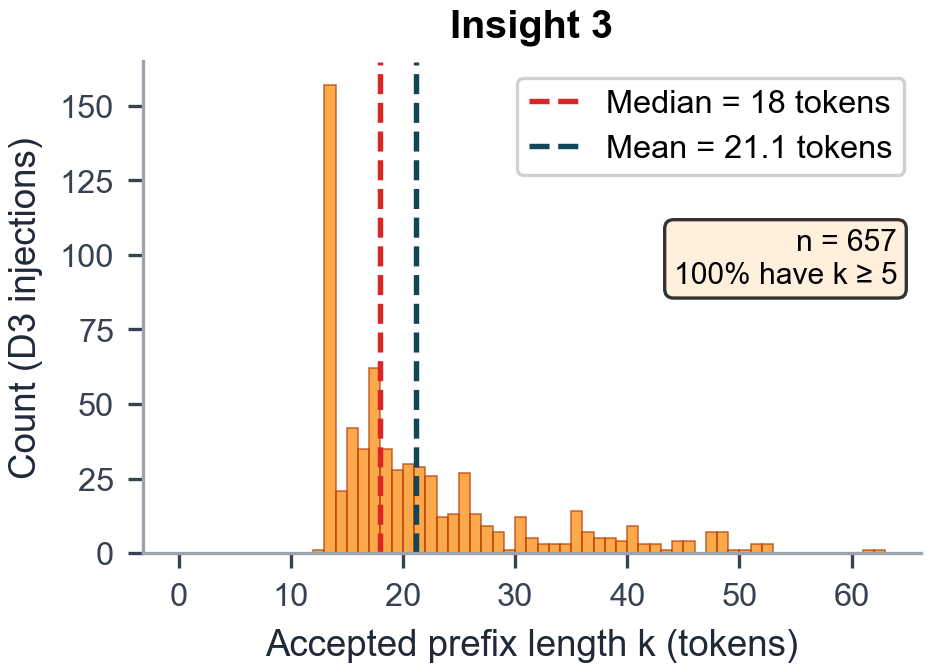
\includegraphics[width=0.93\columnwidth]{figures/fig_insight3_prefix_distribution.png}
  \caption{\textbf{Most rejected probes share recoverable prefixes.}
  On GAIA, the 25th-percentile shared prefix is 14 tokens: 75\% of rejected probes
  share at least 14 tokens with the main tool call.}
  \label{fig:insight3_prefix}
\end{figure}

\parabf{Implication for EQ1.}
Prefix recovery reduces the effective $\Toh$ on the miss branch: instead of discarding
the probe and re-decoding the full tool call from scratch (${\sim}50$ tokens), the system
verifies and accepts $k$ matching tokens and decodes only the $50-k$ suffix.
This is the foundation of D3 (\S\ref{sec:d3}).

\medskip
\begin{tcolorbox}[
  colback=blue!3!white,
  colframe=blue!45!black,
  boxrule=0.45pt,
  arc=1.5pt,
  left=4pt,
  right=4pt,
  top=3pt,
  bottom=3pt
]
\textbf{Summary.}
The three insights establish that self-speculative tool use is \emph{feasible},
\emph{steerable}, and \emph{recoverable}: the model predicts its next tool identity
early, its own confidence signals when to commit, and even rejected probes yield
verified prefixes.
\end{tcolorbox}

\noindent The next section translates these insights into three system mechanisms that
jointly push the operating point toward the EQ1 break-even condition from both sides.
